\begin{frame}{Drivjagt}
    
     \begin{columns}[T]
        \begin{column}{0.58\textwidth}
            \begin{itemize}
                \item \textbf{Semi-aktiv} jagtform – vildtet drives frem til jægerne
                \item Jægeren placeres rundt om området der drives
                \item Jægeren er typisk placeret i jagttårn el lign
                \item Vildtet kommer hurtigt
                \item Større krav til skydefærdigheder
                \item Alle våbentyper i brug
                \item Tæt systematisk drev (drevet går på linie)
                \item Anvendeligt på meget store arealer
                \item Anvendes langsomme jagthunde (terrier, beagle etc)
            \end{itemize}
        \end{column}
        
         \begin{column}{0.4\textwidth}
            \centering
            \vspace{0.5em}
            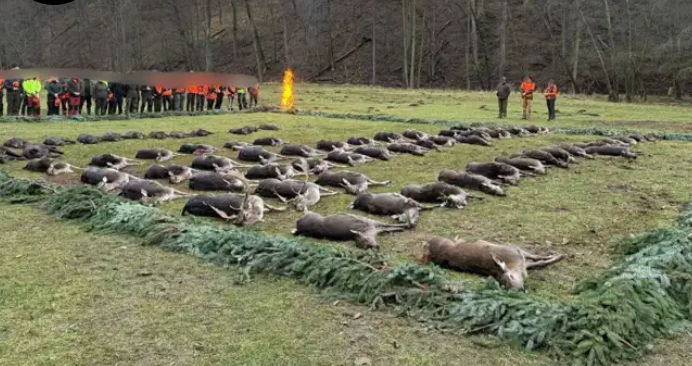
\includegraphics[width=\textwidth,height=0.82\textheight,keepaspectratio]
                {Billeder/Jagtformer/drivjagt}
            % Alternativer – fjern kommentartegn hvis du vil skifte:
            % \includegraphics[width=\textwidth]{highseat-snow-forest-hunter.jpg}
            % \includegraphics[width=\textwidth]{hunter-highseat-morning-mist.jpg}
            % \includegraphics[width=\textwidth]{ansitz-jagttarn-skov.jpg}
        \end{column}
    \end{columns}
    
\end{frame}